% Introduction

\pdfbookmark[1]{Quantitative revolutions}{Introduction}

\chapter{Quantitative revolution(s) in urban science}
\label{chap:quantitative_revolutions}

\begin{flushright}{\slshape    
And the first one now\\
Will later be last\\
For the times, they are a-changin'} \\ \medskip
--- Bob Dylan 
\end{flushright}


\bigskip


\cite{Bairoch:1985} history of cities in french.
\cite{Mumford:1961} history of cities in english.
\cite{Alexander:1965} The city is not a tree.


It is difficult to make a concise summary of what is known and not known about
urban systems. The vast amount of knowledge that has been gathered so far seems
very little in comparison to the bewildering complexity of the object being
studied~\cite{Batty:2008}. Every map, every satellite view, every statistic, every step
in cities elicits a question yet to be answered. What do we have to answer them?
A surprisingly small array of empirical tools and models. A surprisingly small
amount of solid, undisputed empirical facts.\\

\cite{Makse:1995} Modelling urban growth with diffusion limited aggregation
\cite{Rozenfeld:2008} Laws of population growth, using CCA algorithm to define
urban areas.

\cite{Sanders:2011} A good account of the question of scientificity in
geography.

\section{The first quantitative revolution}
\label{sec:the_first_quantitative_revolution}

All started with Christaller and Von T\"unen

Quantification in the US in the 1950-1960. Clear objective to make geography a
science. Berry's student years in the US~\cite{Berry:1993}. 

Strong epistemological component, discipline that is looking for its identity.

Describe objectively the geographical space [Berry,
Haggett]~\cite{Hagget:1966,King:1966,Chorley:1967}
Statistical models~\cite{Brunsdon:1998}
Networks~\cite{Kansky:1963,Haggett:1969}
Seminal text in spatial-quantitative revolution in geography.~\cite{Bunge:1962}

\cite{Tobler:1970} ``Everything is related to everything else. But near things
are more related than others.''

\url{http://www.geog.ucsb.edu/~good/papers/450.pdf}

\begin{equation}
    F_{ij} = C\, \frac{P_i^\alpha\,P_j^\beta}{d_{ij}^\delta}
\end{equation}

Spatial differention
Spatial Interactions (gravity~\cite{Stewart:1948} and intervening opportunities~\cite{Stouffer:1940})
Flows~\cite{Batty:2013}

\section{A second quantitative revolution?}
\label{sec:a_second_quantitative_revolution_}

People can be forgiven for believing that the present time bears any sort of
special character that the past did not. In fact, when we look closely enough,
circumstances are always changing. The change is perpetual. 

In the following, I will discuss the emergence of a term overheard several times
during the past $3$ years, that of 'second quantative revolution' in geography.


Interdisciplinary collaborations already existed, data were already there. So
what is the qualitative difference between the state of the field say $20$ years
ago, and the state of the field as it is now, if any?\cite{Batty:2008,Batty:2012,Batty:2013} seeing the city as flows and networks.


Agent-based models. Physicists have learned to be wary of the attempt to
describe in a deterministic framework the interactions of thousands, billions of
particles. Take a very simple model: the gas of hard spheres. Hard spheres are
simple objects: they have a fixed radius, cannot interpenetrate one another.
Their behaviour is well known, described by Newton's laws of motion, and we can
in theory solve all the equations describing their movements. In fact, we could
imagine, knowing the initial conditions, solve these equations and thus follow
the motion of every single particle (its position and speed) over time. In
practice, computers are way better than we are at doing that, and can easily follow for
us the trajectories of millions of spheres---I have coded that myself as a
student. So we have a very simple system, whose behaviour is perfectly known and
for which we can write exact dynamical equations, thus knowing perfectly its
time evolution at any arbitrary instant in the future. So what? What do we learn
from this simulated motion? What did we understand about the \emph{collective}
motion of spheres that we did not already know performing these simulations?
There is too much information for us to understand. In fact, there is as much
information in these simulations than there is in the original phenomenon, and
our understanding has not improved.
Facing the same questions, the fathers of statistical physics proposed to
extract some simpler, macroscopic information using probabilistic arguments.

Now, regarding social system, the context is even worse. We don't even know the
laws that determine the behaviour of individuals... we do not have the
equivalent of Newton's dynamics to describe the evolution of individuals in time
and their interactions. It is thus difficult what we would gain from simulating
the motions of thousands, millions of them using massive simulations. Even if
the laws were right, what would we learn from these simulations?

    \subsection{New methods?}
    \label{sub:new_methods}

\cite{Batty:1995} comment on Makse et al. DLA approach.
Outsiders applying well-established methods to a new field.

\cite{Stewart:1959} `Physics of population distribution'

\cite{Glass:1971} Cities on a plain.

Simini radiation model~\cite{Simini:2012,Simini:2013} which is nothing else but
applying Stouffer's ideas in a probabilistic context.

DLA approach to modeling urban growth~\cite{Makse:1995}
Percolation on tacts~\cite{Rozenfel:2008} on road networks~\cite{Masucci:2015},
traffic~\cite{Li:2015}
New approaches to spatial networks~\cite{Barthelemy:2011} applied to road
networks~\cite{Barthelemy:2008}.
Out-of-equilibrium models~\cite{Louf:2013_polycentric}

Data analysis putting forth the notion of null, idealised
model~\cite{Louf:2014_scaling}

    \subsection{New data?}
    \label{sub:new_data}

Population Mapping usinf mobile phone data~\cite{Deville:2014}
Lots of talks about new data, but I have used almost none during my thesis.
FourSquare~\cite{Noulas:2012}, Twitter... Credit cards~\cite{Lenormand:2015}

\begin{figure}
    \centering
    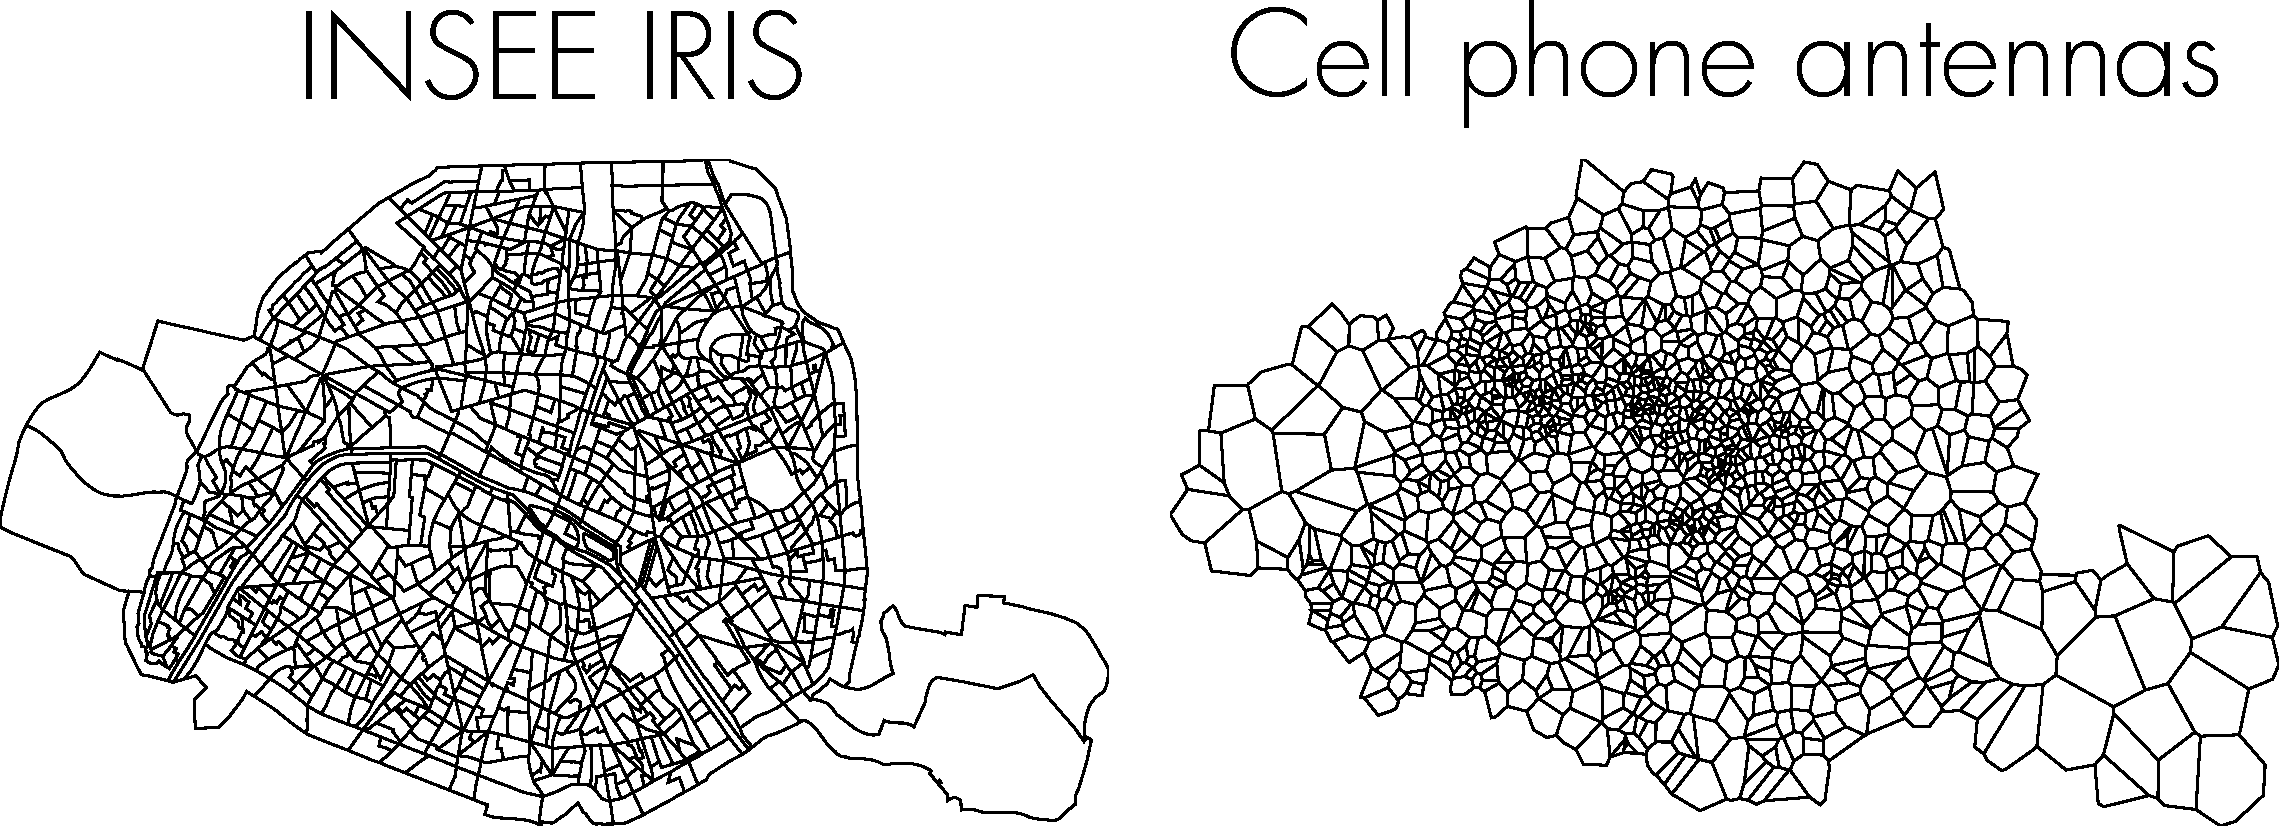
\includegraphics[width=\textwidth]{gfx/chapter-intro/IRIS_phone.pdf}
    \caption{(Left) IRIS zones in Paris, the smallest statistical units defined
    by the national statistics institute, INSEE. (Right) Voronoi tesselation
    built from the position of antennas of a popular french mobile phone carrier.
    There are $40\%$ more antennas than there are IRIS, and they tend to be more
    concentrated in zones of high daily activity (8th and 9th
    arrondissements).\label{fig:IRIS_phone}}
\end{figure}

Mobile phone data are spatially more precise. They give us a \emph{continuous}
information about the flow of individuals within the city, and not only
commuting.

But be careful. If they are ok to monitor aggregate
quantities~\cite{Lenormand:2014}, be careful of
individuals trajectories because sampled in a weird way.

    \subsection{A technological convergence}
    \label{sub:a_technological_convergence} 


